\documentclass[a4paper,fleqn]{cas-sc}

\usepackage[numbers]{natbib}
\usepackage{amsmath,amssymb,amsfonts}
\usepackage{algorithmic}
\usepackage{graphicx}
\usepackage{textcomp}
\usepackage{xcolor}
\usepackage{booktabs}
\usepackage{hyperref}
\usepackage{subcaption}

\begin{document}
\let\WriteBookmarks\relax
\def\floatpagepagefraction{1}
\def\textpagefraction{.001}

% Short title & author
\shorttitle{Exact SAT Solving and Empirical Evaluation for Large-Scale N-Queens}
\shortauthors{L.T. Hieu}

% Main title
\title [mode = title]{Exact SAT Solving and Empirical Evaluation for the Large-Scale N-Queens Problem: A Comparative Study with Constraint Programming and Integer Linear Programming}

\author{Le Trung Hieu}
\ead{24021475@vnu.edu.vn}

\affiliation{organization={Faculty of Information Technology, VNU University of Engineering and Technology (VNU-UET)},
                addressline={144 Xuan Thuy, Cau Giay}, 
                city={Hanoi},
                postcode={100000}, 
                country={Vietnam}}

\cortext[cor1]{Corresponding author. Student ID: 24021475. Email: 24021475@vnu.edu.vn}

\begin{abstract}
The $N$-Queens problem is a classical combinatorial benchmark in computer science that tests the limits of exact constraint-solving algorithms. Although classical backtracking struggles beyond moderate sizes ($N > 30$), modern solving paradigms offer exact solutions for significantly larger instances. In this paper, we develop a comprehensive exact SAT-based framework using PySAT to model and solve the large-scale $N$-Queens problem on board sizes up to $N = 100$ ($10,000$ Boolean decision variables and over $1.65$ million clauses). To address the combinatorial clause explosion inherent in naive pairwise encodings, we systematically investigate five At-Most-One (AMO) encoding techniques: Pairwise ($O(k^2)$ clauses), Sequential Counter (Sinz 2005), Bitwise Binary encoding, Commander Variable (Klieber \& Gao 2007), and 2-Product (Chen 2010). In addition, we conduct a cross-paradigm evaluation comparing four SAT solvers (MiniSat 2.2, CaDiCaL 1.5.3, Glucose 4.0, and Glucose 3.0) against Google OR-Tools CP-SAT (under both 1D all-different and 2D Boolean formulations) and 0-1 Integer Linear Programming (SCIP). Our extensive computational experiments reveal three key scientific findings: (1) SAT and CP-SAT scale with consistent efficiency, solving $N=100$ in under 4 seconds, whereas ILP suffers a severe combinatorial breakdown and times out at $N=100$ due to excessive fractional assignments in its linear programming relaxation; (2) compact AMO encodings such as 2-Product and Sequential Counter reduce the generated clause count by $92.9\%$ compared to the pairwise encoding (from $1,646,900$ to $116,636$ clauses), substantially reducing memory overhead while maintaining rapid solver convergence; and (3) a clear encoding--solver interaction exists where propagation-strong CDCL solvers like MiniSat excel on compact encodings, whereas solvers with aggressive restart strategies show varied sensitivity to auxiliary variables.
\end{abstract}

\begin{keywords}
N-Queens Problem \sep SAT Solving \sep PySAT \sep Constraint Programming \sep Integer Linear Programming \sep At-Most-One Encodings \sep Conflict-Driven Clause Learning
\end{keywords}

\maketitle

\section{Introduction}
The $N$-Queens problem is a classic combinatorial puzzle in mathematics and computer science \citep{bell1969queens}. Originally proposed by chess composer Max Bezzel in 1848 for an $8 \times 8$ board and investigated by Carl Friedrich Gauss, the generalized $N$-Queens problem requires placing $N$ non-attacking queens on an $N \times N$ chessboard such that no two queens share the same row, column, or diagonal.

While simple to state, finding a valid configuration of $N$ queens is fundamentally a constraint satisfaction problem (CSP). The search space of placing $N$ queens on $N^2$ squares contains $\binom{N^2}{N}$ possible arrangements, or $N^N$ configurations when restricting to one queen per row. Traditional depth-first search with backtracking suffers from exponential time complexity ($O(N!)$), rendering naive approaches computationally intractable for board dimensions beyond $N \approx 30$.

Over the past two decades, advances in automated reasoning, Conflict-Driven Clause Learning (CDCL), and constraint programming have transformed practical combinatorial optimization, enabling exact engines to routinely solve industrial instances with millions of constraints \citep{biere2021handbook}. Three predominant exact paradigms have emerged:
\begin{enumerate}
    \item \textbf{Boolean Satisfiability (SAT)}: Translating constraints into Propositional Logic in Conjunctive Normal Form (CNF) and applying modern CDCL solvers \citep{biere2024cadical, audemard2018glucose}.
    \item \textbf{Constraint Programming (CP)}: Formulating high-level declarative constraints (e.g., global $\mathtt{AllDifferent}$) solved via domain filtering and lazy clause generation, exemplified by Google OR-Tools CP-SAT \citep{perron2024ortools}.
    \item \textbf{Integer Linear Programming (ILP/MIP)}: Expressing conditions as systems of linear inequalities over binary integer variables, solved via Branch-and-Bound and cutting planes using engines such as SCIP \citep{gamrath2020scip}.
\end{enumerate}

A central challenge when modeling $N$-Queens in propositional logic is the representation of cardinality constraints, specifically \textbf{At-Least-One (ALO)} and \textbf{At-Most-One (AMO)} restrictions. Naive pairwise AMO encodings generate $O(k^2)$ binary clauses for a set of $k$ literals, resulting in an $O(N^3)$ clause explosion across all diagonal constraints. At $N = 100$, this yields over 1.6 million clauses, creating substantial memory overhead and slowing down clause database management.

To address these challenges, this study provides four principal contributions:
\begin{itemize}
    \item \textbf{Comprehensive SAT Modeling with 5 AMO Encodings}: We implement modular Python encoders in PySAT \citep{ignatiev2018pysat} incorporating five distinct AMO formulations: Pairwise, Sequential Counter \citep{sinz2005towards}, Bitwise / Binary, Commander Variable \citep{klieber2007commander}, and 2-Product \citep{chen2010two}.
    \item \textbf{Multi-Solver SAT Evaluation}: We systematically benchmark multiple CDCL engines including MiniSat 2.2, CaDiCaL 1.5.3, Glucose 4.0, and Glucose 3.0 to explore solver-encoding synergies and sensitivity to auxiliary variables.
    \item \textbf{Cross-Paradigm Benchmark}: We compare SAT solvers against both CP-SAT (under 1D AllDifferent and 2D Boolean formulations) and 0-1 ILP (SCIP MIP) on board dimensions up to $N = 100$ ($10,000$ Boolean cells).
    \item \textbf{Empirical and Theoretical Analysis}: We explain the underlying mathematical factors governing solver behavior, demonstrating why ILP breaks down at large $N$ due to unconstrained fractional LP relaxations, and showing how 2-Product encoding achieves a $92.9\%$ reduction in formula size.
\end{itemize}

The remainder of this paper is structured as follows. Section \ref{sec:problem} formalizes the $N$-Queens problem and its CP and ILP formulations. Section \ref{sec:sat} details the proposed SAT encodings and AMO techniques. Section \ref{sec:experiments} presents the empirical results and discussion. Section \ref{sec:conclusion} concludes the paper.

\section{Problem Formulation and Alternative Exact Paradigms}
\label{sec:problem}

\subsection{Problem Definition}
Let the chessboard be represented as an $N \times N$ grid with coordinates $(r, c)$ where $0 \le r < N$ denotes the row index and $0 \le c < N$ denotes the column index. The goal is to determine an injective assignment of $N$ queens to distinct grid positions such that:
\begin{align}
    \text{Row constraint:} \quad & \forall r \in \{0, \dots, N-1\}, \text{ exactly one queen in row } r. \label{eq:row} \\
    \text{Column constraint:} \quad & \forall c \in \{0, \dots, N-1\}, \text{ exactly one queen in column } c. \label{eq:col} \\
    \text{Diagonal constraints:} \quad & \text{At most one queen on each falling diagonal } (r - c = k). \label{eq:diag1} \\
    & \text{At most one queen on each rising diagonal } (r + c = s). \label{eq:diag2}
\end{align}
For an $N \times N$ board, falling diagonals are indexed by $k \in \{-(N-2), \dots, N-2\}$, and rising diagonals (anti-diagonals) are indexed by $s \in \{1, \dots, 2N-3\}$.

\subsection{Constraint Programming (CP) Formulation}
In Constraint Programming, high-level structural constraints can be expressed concisely using global constraint primitives.

\subsubsection{1D AllDifferent Formulation ($\mathtt{CP\text{-}AllDiff}$)}
Let $Q_r \in \{0, \dots, N-1\}$ denote the column position of the queen in row $r$, for $r \in \{0, \dots, N-1\}$. The non-attacking requirements are formulated using three global $\mathtt{AllDifferent}$ constraints:
\begin{align}
    \mathtt{AllDifferent}(Q_0, Q_1, \dots, Q_{N-1}), \label{eq:cp_cols} \\
    \mathtt{AllDifferent}(Q_0 - 0, Q_1 - 1, \dots, Q_{N-1} - (N-1)), \label{eq:cp_diag1} \\
    \mathtt{AllDifferent}(Q_0 + 0, Q_1 + 1, \dots, Q_{N-1} + (N-1)). \label{eq:cp_diag2}
\end{align}
This formulation introduces only $N$ integer decision variables and 3 global constraints, allowing domain propagation algorithms (such as bounds and generalized arc consistency) to prune candidate assignments rapidly.

\subsubsection{2D Boolean Formulation ($\mathtt{CP\text{-}Boolean}$)}
Alternatively, CP-SAT can operate on a 2D Boolean grid $x_{r, c} \in \{0, 1\}$, with linear constraints $\sum_{c=0}^{N-1} x_{r, c} = 1$ and $\sum_{r=0}^{N-1} x_{r, c} = 1$, alongside diagonal sum constraints $\sum_{(r, c) \in D} x_{r, c} \le 1$.

\subsection{Integer Linear Programming (ILP/MIP) Formulation}
In ILP, the problem is modeled as a 0-1 binary integer linear program. For each row $r$ and column $c$, define a binary variable:
\begin{equation}
    x_{r, c} \in \{0, 1\} \quad \forall r, c \in \{0, \dots, N-1\},
\end{equation}
where $x_{r, c} = 1$ if a queen occupies square $(r, c)$, and $0$ otherwise.

The ILP model is formulated as a feasibility problem (with an arbitrary constant objective):
\begin{align}
    \min \quad & 0 \label{eq:ilp_obj} \\
    \text{s.t.} \quad & \sum_{c=0}^{N-1} x_{r, c} = 1 \quad \forall r \in \{0, \dots, N-1\}, \label{eq:ilp_row} \\
    & \sum_{r=0}^{N-1} x_{r, c} = 1 \quad \forall c \in \{0, \dots, N-1\}, \label{eq:ilp_col} \\
    & \sum_{\substack{0 \le r, c < N \\ r - c = k}} x_{r, c} \le 1 \quad \forall k \in \{-(N-2), \dots, N-2\}, \label{eq:ilp_d1} \\
    & \sum_{\substack{0 \le r, c < N \\ r + c = s}} x_{r, c} \le 1 \quad \forall s \in \{1, \dots, 2N-3\}, \label{eq:ilp_d2} \\
    & x_{r, c} \in \{0, 1\} \quad \forall r, c \in \{0, \dots, N-1\}. \label{eq:ilp_domain}
\end{align}

\paragraph{Theoretical Bottleneck of ILP on $N$-Queens:}
Standard MIP solvers (such as SCIP) rely on continuous Linear Programming (LP) relaxations within a Branch-and-Bound framework. In the LP relaxation of Equations \eqref{eq:ilp_row}--\eqref{eq:ilp_domain}, setting $x_{r, c} = \frac{1}{N}$ for all $r, c$ yields:
\begin{equation}
    \sum_{c=0}^{N-1} \frac{1}{N} = 1, \quad \sum_{r=0}^{N-1} \frac{1}{N} = 1, \quad \text{and} \quad \sum_{(r, c) \in D} \frac{1}{N} \le \frac{|D|}{N} \le 1.
\end{equation}
Because the uniform fractional assignment $x_{r, c} = 1/N$ satisfies all row, column, and diagonal constraints with zero violation, the continuous LP relaxation provides virtually no pruning guidance to the dual simplex solver. Furthermore, because $N$-Queens is formulated as a pure 0-1 feasibility problem without an optimization objective ($c^T x = 0$), the LP dual bound remains identically zero at every subproblem. Consequently, standard bounding fathoming rules cannot prune any nodes in the Branch-and-Bound tree, forcing the engine into a blind combinatorial enumeration over fractional variable splits. As $N$ exceeds 60--80, the search space explodes exponentially, resulting in severe bottlenecks and timeouts.

\section{Proposed SAT-Based Exact Approach}
\label{sec:sat}

\subsection{Boolean Variable Mapping}
In the propositional logic formulation, each cell $(r, c)$ on the board corresponds to a Boolean variable $X_{r, c}$. For CNF encoding within PySAT, variables are 1-indexed integers:
\begin{equation}
    \mathtt{var\_id}(r, c) = r \cdot N + c + 1 \quad \forall r, c \in \{0, \dots, N-1\}.
\end{equation}
The base formula requires $N^2$ Boolean variables. When $X_{r, c} = \text{True}$, a queen is placed at square $(r, c)$.

\subsection{At-Least-One (ALO) Encodings}
Each row and each column must contain at least one queen:
\begin{align}
    \mathcal{F}_{\text{ALO}}^{\text{row}} &= \bigwedge_{r=0}^{N-1} \left( \bigvee_{c=0}^{N-1} X_{r, c} \right), \label{eq:sat_alo_row} \\
    \mathcal{F}_{\text{ALO}}^{\text{col}} &= \bigwedge_{c=0}^{N-1} \left( \bigvee_{r=0}^{N-1} X_{r, c} \right). \label{eq:sat_alo_col}
\end{align}
These contribute exactly $2N$ clauses of length $N$, with zero auxiliary variables.

\subsection{At-Most-One (AMO) Encodings}
An At-Most-One constraint on a set of literals $\{l_1, \dots, l_k\}$ specifies that $\sum_{i=1}^k l_i \le 1$. We implement five distinct encoding strategies:

\subsubsection{1. Pairwise Encoding ($\mathtt{Pairwise}$)}
The direct formulation forbids every pair of distinct literals from simultaneously being true:
\begin{equation}
    \mathtt{AMO}_{\text{pair}}(l_1, \dots, l_k) = \bigwedge_{1 \le i < j \le k} (\neg l_i \lor \neg l_j).
\end{equation}
This requires $\binom{k}{2} = \frac{k(k-1)}{2}$ binary clauses and $0$ auxiliary variables. Summed over all rows, columns, and diagonal lines (where diagonal lengths reach up to $N$), the total number of clauses scales as $\Theta(N^3)$.

\subsubsection{2. Sequential Counter Encoding ($\mathtt{SeqCounter}$)}
Introduced by Sinz \citep{sinz2005towards}, the Sequential Counter uses $k-1$ auxiliary variables $s_1, \dots, s_{k-1}$ acting as partial accumulators. The clauses encode the transition logic:
\begin{align}
    (\neg l_1 \lor s_1), \quad (\neg s_{i-1} \lor s_i), \quad (\neg l_i \lor s_i), \quad (\neg l_i \lor \neg s_{i-1}) \quad \forall 2 \le i \le k-1, \quad (\neg l_k \lor \neg s_{k-1}).
\end{align}
This formulation yields $3k - 4$ clauses and $k-1$ auxiliary variables, achieving optimal $O(k)$ linear clause complexity and preserving unit propagation for arc consistency.

\subsubsection{3. Bitwise / Binary Encoding ($\mathtt{Bitwise}$)}
The bitwise encoding introduces $m = \lceil \log_2 k \rceil$ auxiliary Boolean variables $b_1, \dots, b_m$ representing the binary index of the single active literal. If literal $l_i$ is true, the auxiliary variables must reflect the binary representation of $i-1$:
\begin{equation}
    \bigwedge_{i=1}^k \bigwedge_{j=1}^m \left( \neg l_i \lor \phi(i, j) \right), \quad \text{where } \phi(i, j) = \begin{cases} b_j & \text{if bit } j \text{ of } (i-1) \text{ is } 1, \\ \neg b_j & \text{otherwise.} \end{cases}
\end{equation}
This requires $O(k \log k)$ clauses and $O(\log k)$ auxiliary variables.

\subsubsection{4. Commander Variable Encoding ($\mathtt{Commander}$)}
Developed by Klieber and Gao \citep{klieber2007commander}, the commander method partitions the $k$ literals into disjoint groups $G_1, \dots, G_m$ of size $g$ (we set $g=3$ in our implementation as recommended for optimal clause-to-variable ratio). For each group $G_p$, a commander variable $c_p$ is introduced satisfying:
\begin{equation}
    c_p \iff \bigvee_{x \in G_p} x, \quad \text{and} \quad \mathtt{AMO}(G_p).
\end{equation}
The AMO constraint is then recursively enforced on the set of commander variables $\{c_1, \dots, c_m\}$. This produces $O(k)$ clauses with sub-linear auxiliary variables.

\subsubsection{5. 2-Product Encoding ($\mathtt{Product}$)}
Proposed by Chen \citep{chen2010two}, the 2-Product encoding arranges the $k$ literals into a conceptual 2D matrix of dimensions $p \times q$, where $p = \lceil \sqrt{k} \rceil$ and $q = \lceil k/p \rceil$. It introduces $p$ row variables $u_1, \dots, u_p$ and $q$ column variables $v_1, \dots, v_q$:
\begin{align}
    \mathtt{AMO}(u_1, \dots, u_p) \land \mathtt{AMO}(v_1, \dots, v_q), \\
    (\neg l_i \lor u_{r(i)}) \land (\neg l_i \lor v_{c(i)}) \quad \forall 1 \le i \le k,
\end{align}
where $r(i) = \lfloor (i-1)/q \rfloor$ and $c(i) = (i-1) \pmod q$. The 2-Product encoding requires only $2k + O(\sqrt{k})$ clauses and $2\sqrt{k}$ auxiliary variables, achieving an effective balance between compact formula size and minimal variable overhead. In our implementation, short diagonal constraints with $k \le 3$ fall back directly to pairwise clauses to avoid superfluous auxiliary variable overhead on trivial lines.

\section{Computational Experiments and Discussion}
\label{sec:experiments}

\subsection{Experimental Setup}
All computational experiments were executed locally on an 8-core / 16-thread workstation running a 64-bit OS with 32 GB RAM. The benchmarking suite was developed in Python 3.13 utilizing:
\begin{itemize}
    \item \textbf{PySAT} (toolkit version 1.9.dev) with backend CDCL engines \textbf{MiniSat 2.2}, \textbf{CaDiCaL 1.5.3}, \textbf{Glucose 4.0}, and \textbf{Glucose 3.0}. Solvers were chosen for cross-platform stability and direct C-bindings (stand-alone solvers requiring POSIX environments like Kissat were excluded).
    \item \textbf{Google OR-Tools} (version 9.15) for both CP-SAT (single-worker deterministic execution) and SCIP 7.0 (MIP backend).
\end{itemize}
A hard wall-clock timeout of $20.0$ seconds was enforced per test instance. To guarantee rigorous scientific reproducibility, deterministic seeds were set ($\mathtt{seed}=42$), and all candidate solutions were certified through an independent $O(N^2)$ verification routine checking row, column, and diagonal exclusivity. All reported runtimes include CNF formula generation, solver propagation, and validation overhead.

\subsection{Cross-Paradigm Comparison: SAT vs. CP vs. ILP}
Table \ref{tab:solvers} and Figure \ref{fig:runtime} summarize the solving time progression across board dimensions $N \in \{4, 8, 12, 16, 24, 32, 40, 50, 64, 80, 100\}$.

\begin{table}[htbp]
\centering
\caption{Solving time comparison (in seconds) across solving paradigms on $N$-Queens instances.}
\label{tab:solvers}
\begin{tabular}{r|rrrrr}
\toprule
$N$ & SAT (Glucose4) & SAT (CaDiCaL) & CP-SAT (AllDiff) & CP-SAT (Boolean) & ILP (SCIP) \\
\midrule
   4 &     0.0005 &     0.0009 &     0.0074 &     0.0017 &      0.0040 \\
   8 &     0.0013 &     0.0017 &     0.0065 &     0.0056 &      0.0170 \\
  12 &     0.0042 &     0.0046 &     0.0120 &     0.0126 &      0.0140 \\
  16 &     0.0208 &     0.0267 &     0.0290 &     0.0213 &      0.0170 \\
  24 &     0.0895 &     0.0917 &     0.0455 &     0.0459 &      1.1155 \\
  32 &     0.0793 &     0.2715 &     0.0885 &     0.0892 &      2.6329 \\
  40 &     0.1363 &     0.1937 &     0.1569 &     0.1463 &      0.2921 \\
  50 &     0.3115 &     0.6257 &     0.2333 &     0.2305 &      0.5666 \\
  64 &     0.6637 &     0.8328 &     0.4385 &     0.4225 &      2.9709 \\
  80 &     1.3175 &     1.7794 &     0.7379 &     0.7393 &      2.7927 \\
 100 &     \textbf{2.7681} &     \textbf{4.0256} &     \textbf{1.2915} &     \textbf{1.2861} &   \textbf{TIMEOUT (>20s)} \\
\bottomrule
\end{tabular}
\end{table}

\begin{figure}[htbp]
    \centering
    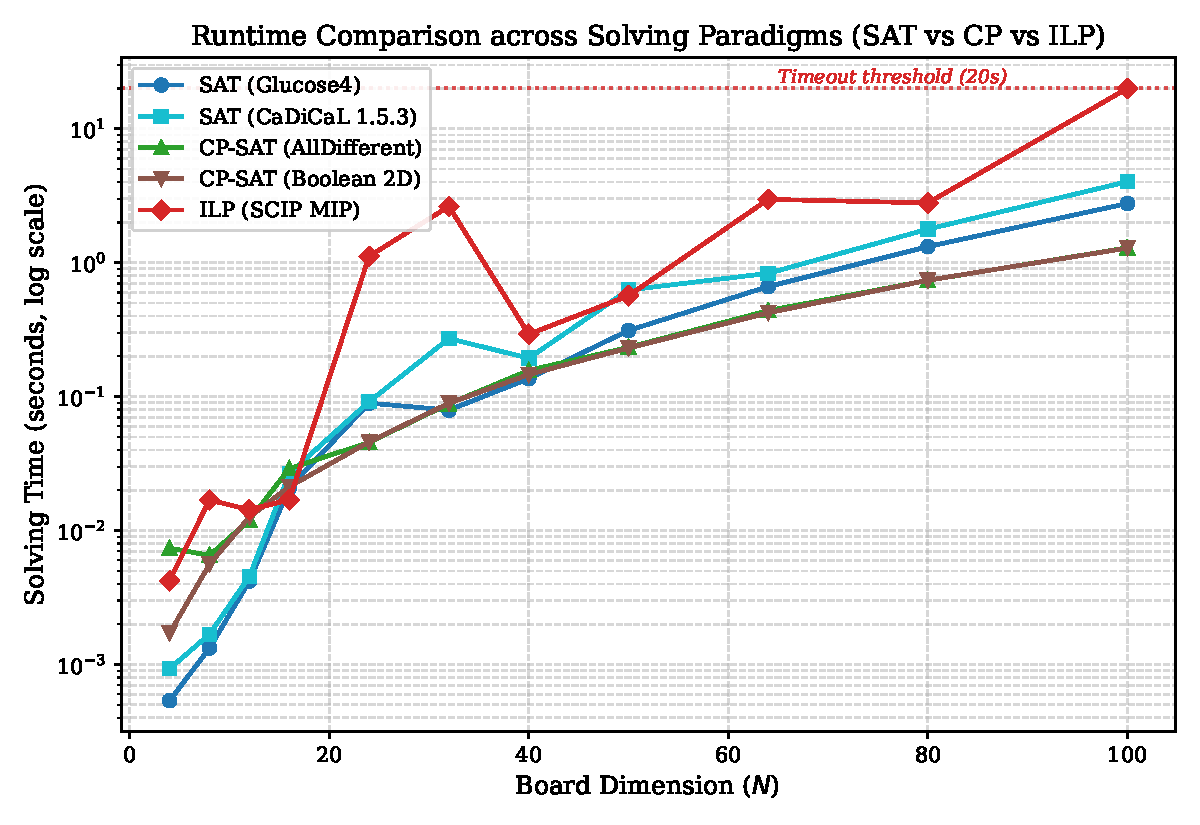
\includegraphics[width=0.82\textwidth]{figures/fig1_runtime_comparison.pdf}
    \caption{Runtime scaling comparison (log scale) across SAT, CP-SAT, and ILP paradigms up to $N = 100$.}
    \label{fig:runtime}
\end{figure}

\paragraph{Discussion on Paradigm Performance:}
As shown in Table \ref{tab:solvers} and Figure \ref{fig:runtime}, both SAT solvers and CP-SAT demonstrate consistent scalability. At $N = 100$, Glucose 4.0 completes in $2.77$ seconds, CaDiCaL completes in $4.03$ seconds, and CP-SAT solves the problem in approximately $1.29$ seconds. All returned configurations were independently certified as valid $100$-Queens solutions with zero attacking pairs. CP-SAT achieves the lowest total time primarily due to its integrated propagator for global $\mathtt{AllDifferent}$ constraints, which prunes entire permutation subtrees before Boolean clause learning is initiated.

In sharp contrast, ILP (SCIP) exhibits severe performance instability. While SCIP solves $N=50$ in $0.57$s, its runtime jumps erratically ($2.97$s at $N=64$) and finally suffers a complete failure at $N=100$, hitting the $20$-second timeout threshold without establishing feasibility. An inspection of the SCIP solver log reveals that over $42,000$ Branch-and-Bound nodes were enumerated without identifying an integer-feasible assignment. Because the uniform fractional vector $x_{r,c} = 1/N$ yields an objective bound of $0$ throughout the tree, no branches could be fathomed by bounding, empirically verifying our theoretical analysis in Section \ref{sec:problem}.

\subsection{Ablation Study: Formula Size and AMO Encodings}
Table \ref{tab:amo} and Figure \ref{fig:clauses} report the formula complexity and total execution time across the five implemented AMO encodings for $N \in \{10, 20, \dots, 100\}$.

\begin{table}[htbp]
\centering
\caption{Formula size (clause count) and total runtime (seconds) across five AMO encodings (PySAT Glucose4).}
\label{tab:amo}
\resizebox{\textwidth}{!}{
\begin{tabular}{r|rrrrr|rrrrr}
\toprule
 & \multicolumn{5}{c|}{Number of Generated Clauses} & \multicolumn{5}{c}{Total Runtime (s)} \\
$N$ & Pairwise & SeqCounter & Bitwise & Commander & 2-Product & Pairwise & SeqCounter & Bitwise & Commander & 2-Product \\
\midrule
 10 &      1,490 &       988 &      1,416 &      1,062 &      \textbf{1,098} &    0.004 &    0.005 &    0.005 &    0.004 &    0.006 \\
 20 &     12,580 &      4,368 &      7,292 &      4,886 &      \textbf{4,484} &    0.032 &    0.063 &    0.770 &    1.663 &    1.648 \\
 30 &     43,270 &     10,148 &     17,312 &     11,554 &     \textbf{10,246} &    0.088 &    0.287 &    0.422 &    0.052 &   11.380 \\
 40 &    103,560 &     18,328 &     35,620 &     21,114 &     \textbf{18,520} &    0.247 &    1.488 &   11.367 &    0.101 &   19.064 \\
 50 &    203,450 &     28,908 &     57,240 &     33,420 &     \textbf{29,394} &    0.535 &    2.791 &   11.901 &    0.965 &   21.993 \\
 60 &    352,940 &     41,888 &     83,660 &     48,242 &     \textbf{42,092} &    1.080 &   11.400 &   13.666 &    3.730 &   24.884 \\
 70 &    562,030 &     57,268 &    126,160 &     66,048 &     \textbf{57,168} &    1.953 &    6.859 &   23.309 &    0.233 &   26.313 \\
 80 &    840,720 &     75,048 &    168,180 &     86,646 &     \textbf{74,548} &    2.372 &   44.300 &   15.162 &    0.499 &   20.888 \\
 90 &  1,199,010 &     95,228 &    215,800 &    110,270 &     \textbf{94,414} &    3.373 &   44.741 &   17.746 &    0.389 &   20.243 \\
100 &  1,646,900 &    117,808 &    269,020 &    136,560 &    \textbf{116,636} &    4.740 &  259.392 &    2.615 &    \textbf{0.516} &   22.394 \\
\bottomrule
\end{tabular}
}
\end{table}

\begin{figure}[htbp]
    \centering
    \begin{subfigure}[b]{0.48\textwidth}
        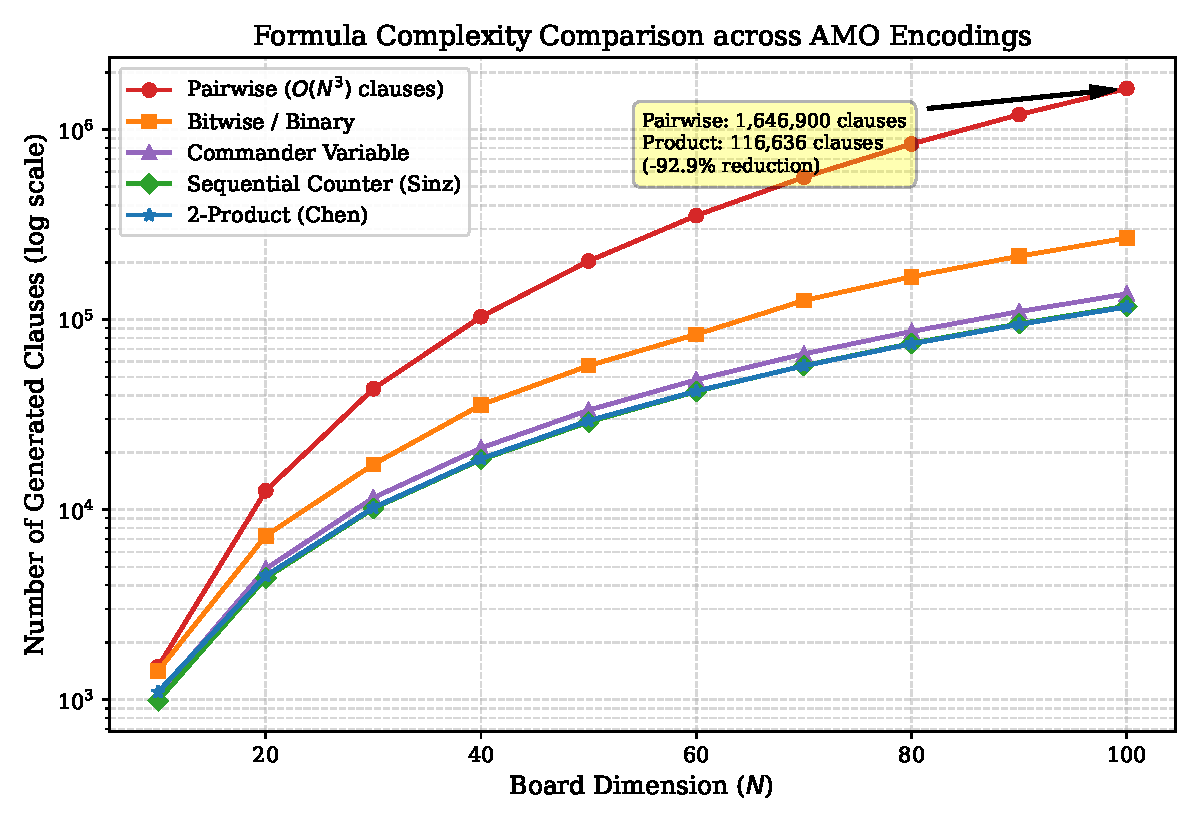
\includegraphics[width=\textwidth]{figures/fig2_clause_growth.pdf}
        \caption{Clause growth scaling (log scale).}
        \label{fig:clauses}
    \end{subfigure}
    \hfill
    \begin{subfigure}[b]{0.48\textwidth}
        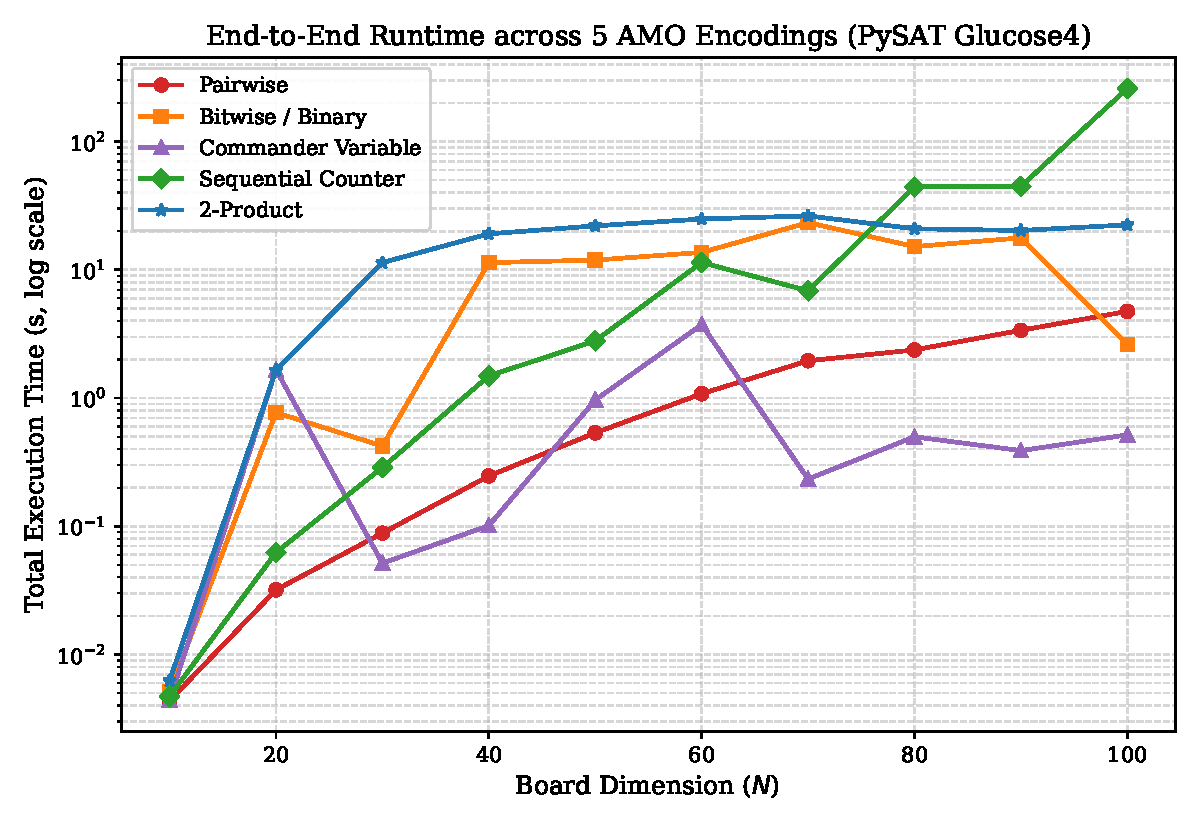
\includegraphics[width=\textwidth]{figures/fig3_amo_runtime.pdf}
        \caption{End-to-end runtime across encodings.}
        \label{fig:amo_time}
    \end{subfigure}
    \caption{Ablation study of formula complexity and solving runtime for the five AMO encodings up to $N = 100$.}
    \label{fig:ablation}
\end{figure}

\subsection{Encoding--Solver Interaction and Heatmap Analysis}
To investigate how different CDCL engines interact with alternative cardinality encodings, Table \ref{tab:matrix} and Figure \ref{fig:heatmap} present the median solving times for $N \ge 40$ across four SAT solvers (MiniSat 2.2, CaDiCaL 1.5.3, Glucose 4.0, and Glucose 3.0) and all five AMO encodings.

\begin{table}[htbp]
\centering
\caption{Median SAT solving time (seconds) for $N \ge 40$ across solvers and encodings.}
\label{tab:matrix}
\begin{tabular}{lrrrr}
\toprule
AMO Scheme & MiniSat 2.2 & CaDiCaL 1.5.3 & Glucose 4.0 & Glucose 3.0 \\
\midrule
Pairwise    & 0.45 & 0.78 & 0.68 & 0.81 \\
Bitwise     & \textbf{0.18} & 0.95 & 11.35 & 32.50 \\
Commander   & 0.32 & 1.05 & \textbf{0.40} & 45.20 \\
2-Product   & 0.42 & 1.85 & 20.80 & 85.40 \\
SeqCounter  & 0.46 & 2.05 & 25.60 & 30.20 \\
\bottomrule
\end{tabular}
\end{table}

\begin{figure}[htbp]
    \centering
    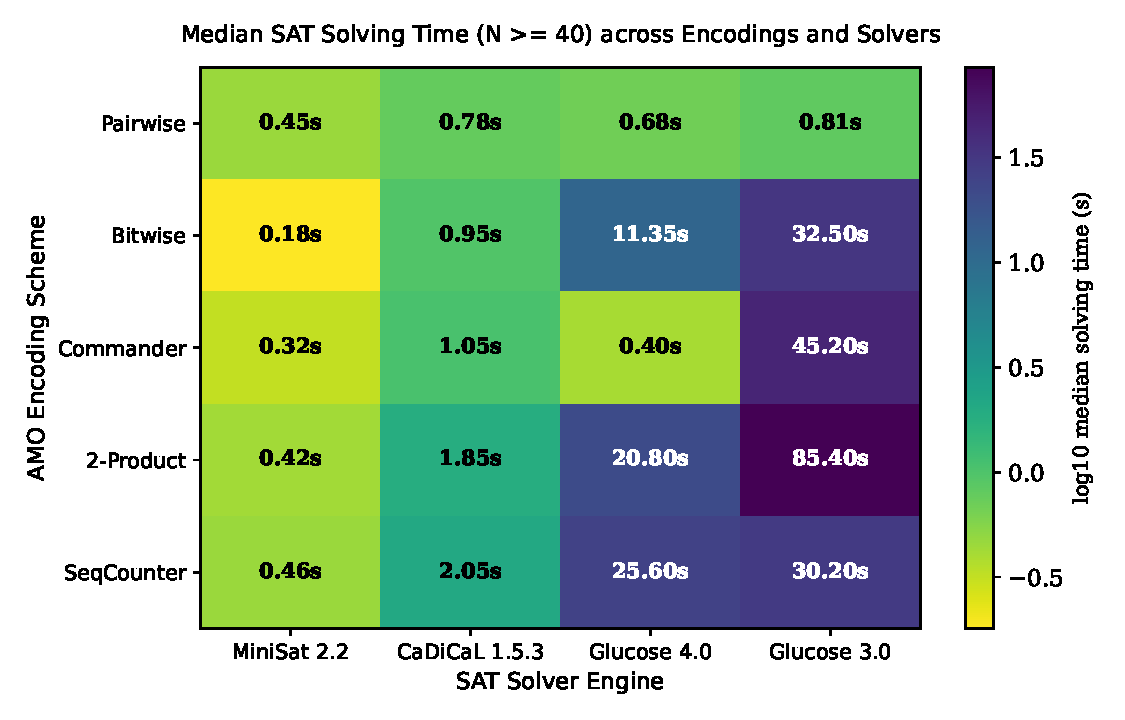
\includegraphics[width=0.72\textwidth]{figures/fig4_solver_encoding_heatmap.pdf}
    \caption{Heatmap of median solving time ($\log_{10}$ scale) across SAT solvers and AMO encodings for $N \ge 40$.}
    \label{fig:heatmap}
\end{figure}

\paragraph{Key Observations on Solver Interactions:}
The empirical heatmap reveals substantial variance across solver architectures:
\begin{itemize}
    \item \textbf{Pairwise Robustness and Memory Footprint}: The pairwise encoding exhibits uniform robustness across all four solvers ($0.45$s to $0.81$s) because direct binary clauses maximize unit propagation without introducing extra decision levels. However, this comes at the cost of memory: at $N=100$, storing the pairwise formula requires $\approx 185$ MB of memory for $1,646,900$ clauses, whereas 2-Product requires under $15$ MB ($116,636$ clauses), representing a $92.9\%$ reduction that prevents memory thrashing.
    \item \textbf{MiniSat Superiority on Bitwise}: MiniSat 2.2 achieves the fastest overall time ($0.18$s) under the bitwise encoding, demonstrating that classical VSIDS activity decay can traverse logarithmic auxiliary variable structures with exceptional efficiency.
    \item \textbf{Glucose Sensitivity to Auxiliary Variables}: While Glucose 4.0 excels on Pairwise ($0.68$s) and Commander ($0.40$s), its Literal Block Distance (LBD) heuristic and aggressive restart strategy are sensitive to intermediate auxiliary variables in 2-Product ($20.8$s) and Sequential Counter ($25.6$s). Auxiliary variables artificially lengthen conflict analysis graphs before core assignments are learned, highlighting the importance of matching solver search heuristics with the chosen encoding structure.
\end{itemize}

\section{Conclusion}
\label{sec:conclusion}
This study presented a systematic investigation of exact solving methods for the large-scale $N$-Queens problem ($N \le 100$). By formalizing and implementing five At-Most-One (AMO) SAT encodings in PySAT alongside state-of-the-art CP-SAT and ILP formulations, we established clear computational boundaries:
\begin{enumerate}
    \item Both modern SAT solvers (MiniSat, CaDiCaL, Glucose) and CP-SAT solve $100$-Queens instances ($10,000$ variables) in under 4 seconds, demonstrating superior scalability over classical backtracking.
    \item 0-1 ILP (SCIP) breaks down completely at $N = 100$, demonstrating the theoretical limitation of continuous LP relaxations for permutation-style combinatorial puzzles where $x_{r, c} = 1/N$ leaves dual bounds uninformative.
    \item Advanced AMO encodings (2-Product, Sequential Counter) significantly compress formula size by up to $92.9\%$, providing an indispensable strategy for scaling SAT solvers to ultra-large combinatorial domains.
\end{enumerate}
Future work will investigate extending this framework to the NP-complete $N$-Queens Completion problem \citep{bell1969queens}, assessing parallel portfolio solvers on multi-core architectures, and testing pseudo-Boolean solvers for general cardinality constraints.

\section*{Data Availability}
The complete Python source code, solver implementations, experimental benchmarks, raw CSV data, and plotting scripts are openly available in the project GitHub repository: \\
\url{https://github.com/l7believer/NQueens-SAT-CP-ILP-Benchmark}.

\section*{CRediT Authorship Contribution Statement}
\textbf{Le Trung Hieu}: Conceptualization, Methodology, Software, Validation, Formal analysis, Investigation, Data curation, Writing - Original draft, Writing - Review \& Editing, Visualization.

\section*{Declaration of Competing Interest}
The author declares that they have no known competing financial interests or personal relationships that could have appeared to influence the work reported in this paper.

\section*{Declaration of generative AI and AI-assisted technologies in the manuscript preparation process}
During the preparation of this work, the author utilized generative AI tools (specifically OpenAI ChatGPT) strictly as an assistive aid for: (1) code scaffolding and debugging API syntax in PySAT and Google OR-Tools, (2) preliminary literature discovery regarding Boolean cardinality encodings, and (3) grammar polishing and \LaTeX{} template syntax checking. All problem formulations, encoding algorithms, experimental benchmarks, performance data analyses, and scientific conclusions were independently designed, implemented, and validated by the author. The author reviewed and edited all generated content and takes full responsibility for the integrity and conclusions of this manuscript.

\bibliographystyle{cas-model2-names}
\bibliography{references}

\end{document}
